\chapter{Przetwarzanie danych}
\label{cha:budowaGrafu}

Przedstawione w rozdziale \ref{cha:pozyskiwanieTresci} oprogramowanie umożliwia efektywne pobieranie wiadomości z sieci, daje możliwość odświeżania posiadanych informacji
i roszerzania kolekcji dokumentów o nowe pozycje. Rzadko jednak przechowywanie danych jest celem samym w sobie. Oprócz programów archiwizujących, zazwyczaj pobranie dokumentu jest pierwszym
etapem algorytmu przetwarzającego dane. Dobrym przykładem jest wyszukiwarka internetowa, w której ważna jest zarówno ilość pobranych stron i ich reprezentatywność na tle całej sieci, jak
i algorytm oceny przydatności poszczególnych dokumentów.

Jednym z najważniejszych aspektów tworzenia dobrego silnika przetwarzającego dane jest wybór odpowiedniej, przystosowanej do
wykonywanego zadania, struktury danych. Literatura poferuje szeroki wachlarz silników bazodanowych, od relacyjnych, po bazy NoSQL. Niniejsza praca ma na celu przedstawienie wykorzystania
struktur grafowych do przechowywania danych ściągniętych z sieci. W tym rozdziale poruszone zostaną pokrótce zalety przedstawienia danych w postaci grafu i omówiony zostanie pewien 
szczególny rodzaj grafu, jakim jest asocjacyjna grafowa struktura danych(AGDS) \cite[s. 108]{Horzyk}. 

\section{Wykorzystanie grafu jako struktury danych}
\label{section:graf}

%Formalnie, graf jest to uporządkowana para \( G = (V,E)\) zbiorów wierzchołków -\(V\) i krawędzi - \(E\), dla których \(E \subseteq [V]^2 \). Oznacza to, iż 
%czyli elementy \(E\) są 2 - elementowymi podzbiorami \(V\) \cite{teoriaGraf}. 
 
Struktura grafu wyjątkowo dobrze oddaje bezpośrednie relacje pomiędzy elementami w niej zawartymi, ponadto da się przedstawić w prosty i intuicyjny 
sposób. Klasycznymi przykładami problemów matematycznych przedstawiancyh w postaci grafu są np. problem mostów w Królewcu(problem decyzyjny, określający
czy w danym grafie istnieje cykl Eulera), czy problem komiwojażera. Wraz z rozwojem internetowych sieci społecznościowych zaczęto zwracać uwagę na 
możliwości wykorzystania grafów w celu badania sieci, czy przeszukiwania informacji w nich zawartych - przykładem takiego zastosowania jest 
usługa Graph Search udostępniana prez portal Facebook -\url{https://www.facebook.com/about/graphsearch}. Poniżej przedstawione zostaną cechy grafu,
które decydują o jego rosnącej popularności \cite{graphDb}:
\begin{enumerate}
    \item \textbf{Szybkość} - wyszukanie danych o relacjach pojedynczego wierzchołka nie wymaga kosztownych operacji \emph{join} na całych tabelach,
    dostęp do danych jest szybki. Nawet w przypadku wzrostu liczby wierzchołków, czas wykonywania większości zapytań nie zmienia się, ponieważ dotyczą
    one jedynie fragmentu bazy.
    \item \textbf{Elastyczność} - graf nie wymaga tak dogłębnego określenia struktury bazy, jak tradycyjna baza relacyjna. Dodawanie nowych relacji, 
    węzłów, czy podgrafów jest stosunkowo proste i nie wymaga migracji. Dzięki temu, możliwy jest bardziej dynamiczny rozwój aplikacji opartych o bazy grafowe.
\end{enumerate}

Warto wspomnieć, iż istnieją aplikacje, dla których bazy grafowe są niezastapione, choćby ze względu na ograniczenia szybkości baz relacyjnych. Przykładem na to jest
przytoczone w \cite{neo4jAction} oprogramowanie szukające relacji typu ``znajomy znajomego'' w bazie użytkowników sieci społecznościowych. Dla około~1~000~000
użytkowników posiadających średnio po 50 kontaktów, baza grafowa - w tym przypadku Neo4j - okazała się szybsza o kilka rzędów wielkości od tradycyjnej bazy
relacyjnej.

\begin{table}[h!]
\centering
\label{tabela:neo4jAwesome}
\caption{Poszukiwanie ``znajomych znajomych'' w bazie relacyjnej i grafowej}
\begin{tabular}{cccc}
\hline
&  \multicolumn{2}{c}{Czas wykonania [s]} &\\
\cline{2-3}
Zagnieżdżenie & RDBMS & Baza grafowa & Zwrócone rekordy\\
\hline
2 & 0.16 & 0.01 & \(\approx\) 2500 \\
3 & 30.267 & 0.168 & \(\approx\) 110 000\\
4 & 1543.505 & 1.359 & \(\approx\) 600 000\\
5 & nieukończono & 2.132 & \(\approx\) 800 000\\ 
\hline
\end{tabular}
\end{table}


%-----------------------------------------------------------------

\section{Asocjacyjne grafowe struktury danych}
\label{sec:agds}
Często \textbf{asocjacją} (skojarzeniem) nazywa się powiązanie ze sobą dwóch lub więcej zdefiniowanych wcześniej elementów. Zgodnie z \cite[s. 47]{Horzyk} 
tą definicję można rozszerzyć, opierając się na obserwacji biologicznych organizmów żywych. Zauważono, iż niektóre organizmy mają umiejętność
powiązywania dostepnych dla siebie danych w skomplikowane sieci zależnośc(asocjacji). Do kryteriów, wg których skojarzenia są budowane, należą:
\begin{enumerate}
    \item Miara podobieństwa. 
    \item Odległość w czasie recepcji informacji.
    \item Kontekst, w którym informacje się pojawiły.
\end{enumerate}
W związku z tym, iż organizmy żywe ciągle pozostają pod wieloma względami niedoścignione w wielu dziedzinach(np. jak analiza obrazu, czy mowy, gdy mowa o 
człowieku), postanowiono podjąć próbę konstrukcji sztucznych systemów asocjacycjnych, naśladujących te występujące w naturze.

\subsection{Definicja}
\label{subsec:assocDef}

Poniższe definicje \cite[s. 53-56]{Horzyk} opisują podstawowe elementy systemu asocjacyjnego. Na ich potrzebę można przyjąć, iż ma on ogólną budowę grafu mieszanego,
w którego węzłach umieszczone są sztuczne neurony, a krawędzie odpowiadają synapsom(połączeniom międzyneuronalnym):

\begin{definicja}
    \textbf{Relacją(asocjacyjną)} nazywamy każdą relację pomiędzy obiektami(węzłami) zapamiętywanymi i kojarzonymi ze sobą przez system asocjacyjny.
\end{definicja}

\begin{definicja}
    Powiązania łączące podobne i bliskie dane, ich kombinacje i układy nazywane są \textbf{powiązaniami asocjacyjnego podobieństwa} - \textbf{ASIM}.
\end{definicja}

ASIM ma miejsce wtedy, gdy system przetwarza informacje podobne, jednorodne dane lub ich układy.

\begin{definicja}
    Powiązania łączące dane, ich powiązania i układy, które następują chronologicznie po sobie lub przestrzennie ze sobą sąsiadują są nazywane
    \textbf{powiązaniami asocjacyjnego następstwa} - \textbf{ASEQ}.
\end{definicja}

ASEQ związany jest z powtarzającymi się sekwencjami danych lub danymi pobudzającymi ten sam fragment grafu.

\begin{definicja}
    Powiązania łączące dane, ich kombinacje i układy w taki sposób, że zwykle samodzielnie nie prowadzą do aktywacji neuronów stanowiących węzły
    grafu, lecz stanowią tylko pewien kontekst wspomagający ewentualne wywołanie przyszłych aktywnych reakcji neuronów, wywołanych dopiero na skutek
    następnych procesów skojarzeniowych, nazywa się \textbf{powiązaniami asocjacyjnego kontekstu} - \textbf{ACON}.
\end{definicja}

ACON to powiązanie niemal analogiczne do ASEQ, z tą różnicą, iż nie skutkuje ono od razu aktywacją neuronu, a pełni tylko funkcję wspomagającą.

\begin{definicja}
    Bezpośrednie połączenia od receptorów lub neuronów przekazujących dane wejściowe do neuronu, który reprezentuje niektóre kombinacje lub układy 
    zbudowane z tych danych to \textbf{powiązania asocjacyjnego definiowania} - \textbf{ADEF}.
\end{definicja}

Powstają one w wyniku oddziaływania wielu neuronów, receptorów lub neuronów receptorycznych na ten sam neuron.

\begin{definicja}
    \label{def:agds}
    \textbf{Grafowa asocjacyjna struktura danych AGDS} (ang. \emph{associative graph data structure}) to graf umożliwiający przechowywanie wartości danych
    i ich kombinacji wraz z uproszczoną reprezentacją ich asocjacyjnego podobieństwa(ASIM), asocjacyjnego następstwa(ASEQ) i asocjacyjnego definiowania(ADEF), jakie wystepują między nimi.
\end{definicja}

W zapisie formalnym struktura AGDS jest to uporządkowana siódemka \linebreak \(AGDS = (VV, VR, VS, VC, ESIM, ESEQ, EDEF) \) \cite[s. 109]{Horzyk}, gdzie:

\begin{description}
    \item \(VV\) - zbiór wierzchołków reprezentujących poszczególną wartość (ang. \emph{value vertex}),
    \item \(VR\) - zbiór wierzchołków reprezentujących przedział wartości (ang. \emph{range vertex}),
    \item \(VS\) - zbiór wierzchołków reprezentujących podzbiór wartości (ang. \emph{subset vertex}),
    \item \(VC\) - zbiór wierzchołków reprezentujących kombinację wartości (ang. \emph{combination vertex}),
    \item \(ESIM\) - zbiór krawędzi nieskierowanych, łączących asocjacyjnie podobne wierzchołki,
    \item \(ESEQ\) - zbiór krawędzi skierowanych łączących asocjacyjnie nasępne wierchołki,
    \item \(EDEF\) - zbiór krawędzi dwustronnie skierowanych łączących wierzchołek definiujący z wierzchołkiem definiowanym w taki sposób,
                     iż etykieta (waga) określa przejście od jednego, do drugiego wierzchołka.
\end{description}

Krawędzie dwustronnie skierowane można przedstawić również jako parę krawędzi jednostronnie skierowanych.

Struktura AGDS jest statyczna i z tego względu nie można za jej pomocą modelować innych relacji asocjacyjcnych przedstawionych w \cite{Horzyk}.
Typowo dane odwzorowywane są w niej za pomocą wierzchołków grafu(neuronów), natomiast krawędzie przedstawiają informację o ich wzajemnym powiązaniu, bazującym np.~na~częstotliwości
występowania. Praca z grafem polega bądź na wykorzystaniu istniejących algorytmów przeszukiwania grafu w celu uzyskania interesujących informacji, bądź
na przekstałceniu struktury AGDS do postaci grafów AANG - \textbf{aktywnych asocjacyjnych grafów neuronowych} i stosowaniu algorytmów asocjacyjnych.
Ważnym założeniem charakterystycznym dla grafów asocjacyjnych jest unikalność informacji przechowywanej w węzłach. 

\subsection{Przedstawienie danych w postaci AGDS}
Na schemacie \ref{graph:relacyjne} przedstawiona jest struktura pewnej relacyjnej bazy danych. Składa się ona z dwóch tabel modelujących relacje:~
użytkowników i prezentów, jakie otrzymali. 

\begin{figure}[!h]
    \centering
    \label{graph:relacyjne}
    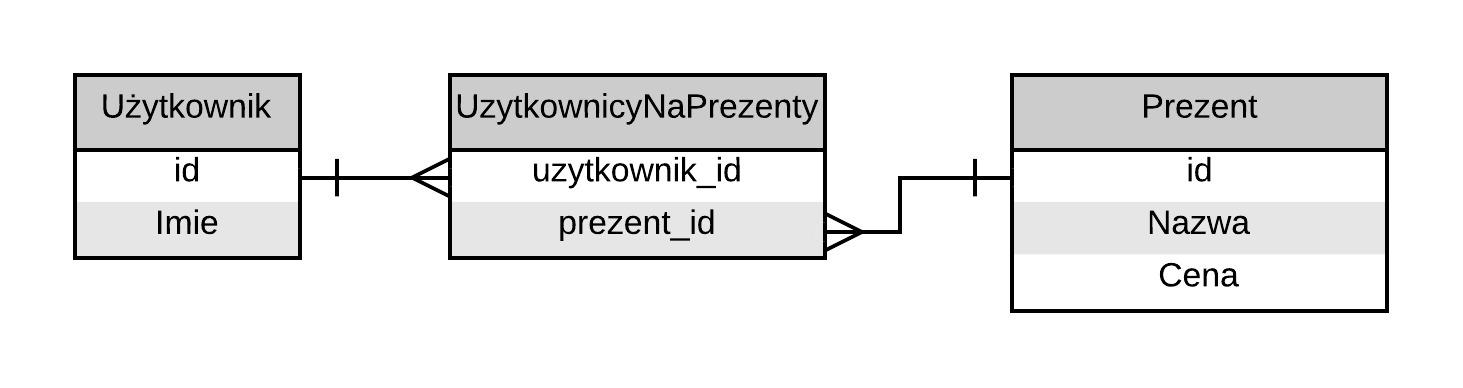
\includegraphics[scale=0.3]{baza_prezenty}
    \caption{Schema relacyjnej bazy danych przedstawiająca użytkowników i prezenty, jakie otrzymali}
\end{figure}

\begin{table}
\centering
\caption{Przykładowe dane}
\begin{tabular}{ccc}

\begin{tabular}[t]{| c | c |}
\hline
id & Imię \\
\hline
1 & Mariusz \\
\hline
2 & Weronika \\
\hline
3 & Bazyl \\
\hline
\end{tabular}
&
\begin{tabular}[t]{| c | c |}
\hline
uzytkownik\_id & prezent\_id \\
\hline
1 & 1 \\
\hline
1 & 2 \\
\hline
2 & 2 \\
\hline
2 & 3 \\
\hline
3 & 4 \\
\hline
3 & 1\\
\hline
3 & 5 \\
\hline
\end{tabular}
&
\begin{tabular}[t]{| c | c | c | }
\hline
id & Nazwa & Cena\\
\hline
1 & Zegarek & 1500 \\
\hline
2 & Łyżwy & 300 \\
\hline
3 & Zegarek & 300 \\
\hline
4 & Łyżwy & 100 \\
\hline
5 & Sweter & 60 \\
\hline
\end{tabular}
\end{tabular}
\end{table}

\begin{table}
\label{tabela:join}
    \centering
    \caption{Tabela joinująca, zaprezentowana w celu zilustrowania danych}
    \begin{tabular}{| c | c | c |}
        \hline
        Imie & Nazwa Prezentu & Cena \\
        \hline
        Mariusz & Zegarek & 1500 \\
        \hline
        Mariusz & Łyżwy & 300 \\
        \hline
        Weronika & Łyżwy & 300 \\
        \hline
        Weronika & Zegarek & 300 \\
        \hline
        Bazyl & Sweter & 60 \\
        \hline
        Bazyl & Zegarek & 1500 \\
        \hline
        Bazyl & Łyżwy & 100 \\
        \hline
    \end{tabular}

\end{table}

W przypadku używania relacyjnej struktury danych, łatwo zauważyc dwa istotne problemy. Gdy wprowadzona zostaje normalizacja, zazwyczaj informacje nie są duplikowane pomiędzy
tabelami, wszystkie zależności wyrażone są w postaci relacji. Jednak operacje na takich zbiorach danych łączą się z koniecznością używania złączeń, które w wypadku
tabel o wielu rekordach dają duży narzut obliczeniowy(jak przedstawiono na \ref{tabela:neo4jAwesome}). W razie świadomej denormalizacji, jak w przypadku zilustrowanym w tabeli
\ref{tabela:join}, mogą występować problemy związane z niespójnością danych. Trudno wprowadzać do takiej struktury zmiany, jest ona podatna na różne anomalie.

Na rysunku \ref{graph:agds} przedstawiony jest ten sam zbiór danych, ale z wykorzystaniem struktur AGDS. Niewątpliwą zaletą takiego przedstawienia jest możliwość natychmiatowego
otrzymania informacji o relacjach zachodzących między poszczególnymi obieketami. Otrzymanie infomracji o liscie prezentów użytkownika, wszystkich użytkownikach posiadających
ten sam prezent, czy średniej cenie prezentu danego typu jest bardzo proste i niewymagające obliczeniowo.

\begin{figure}[!h]
    \label{graph:agds}
    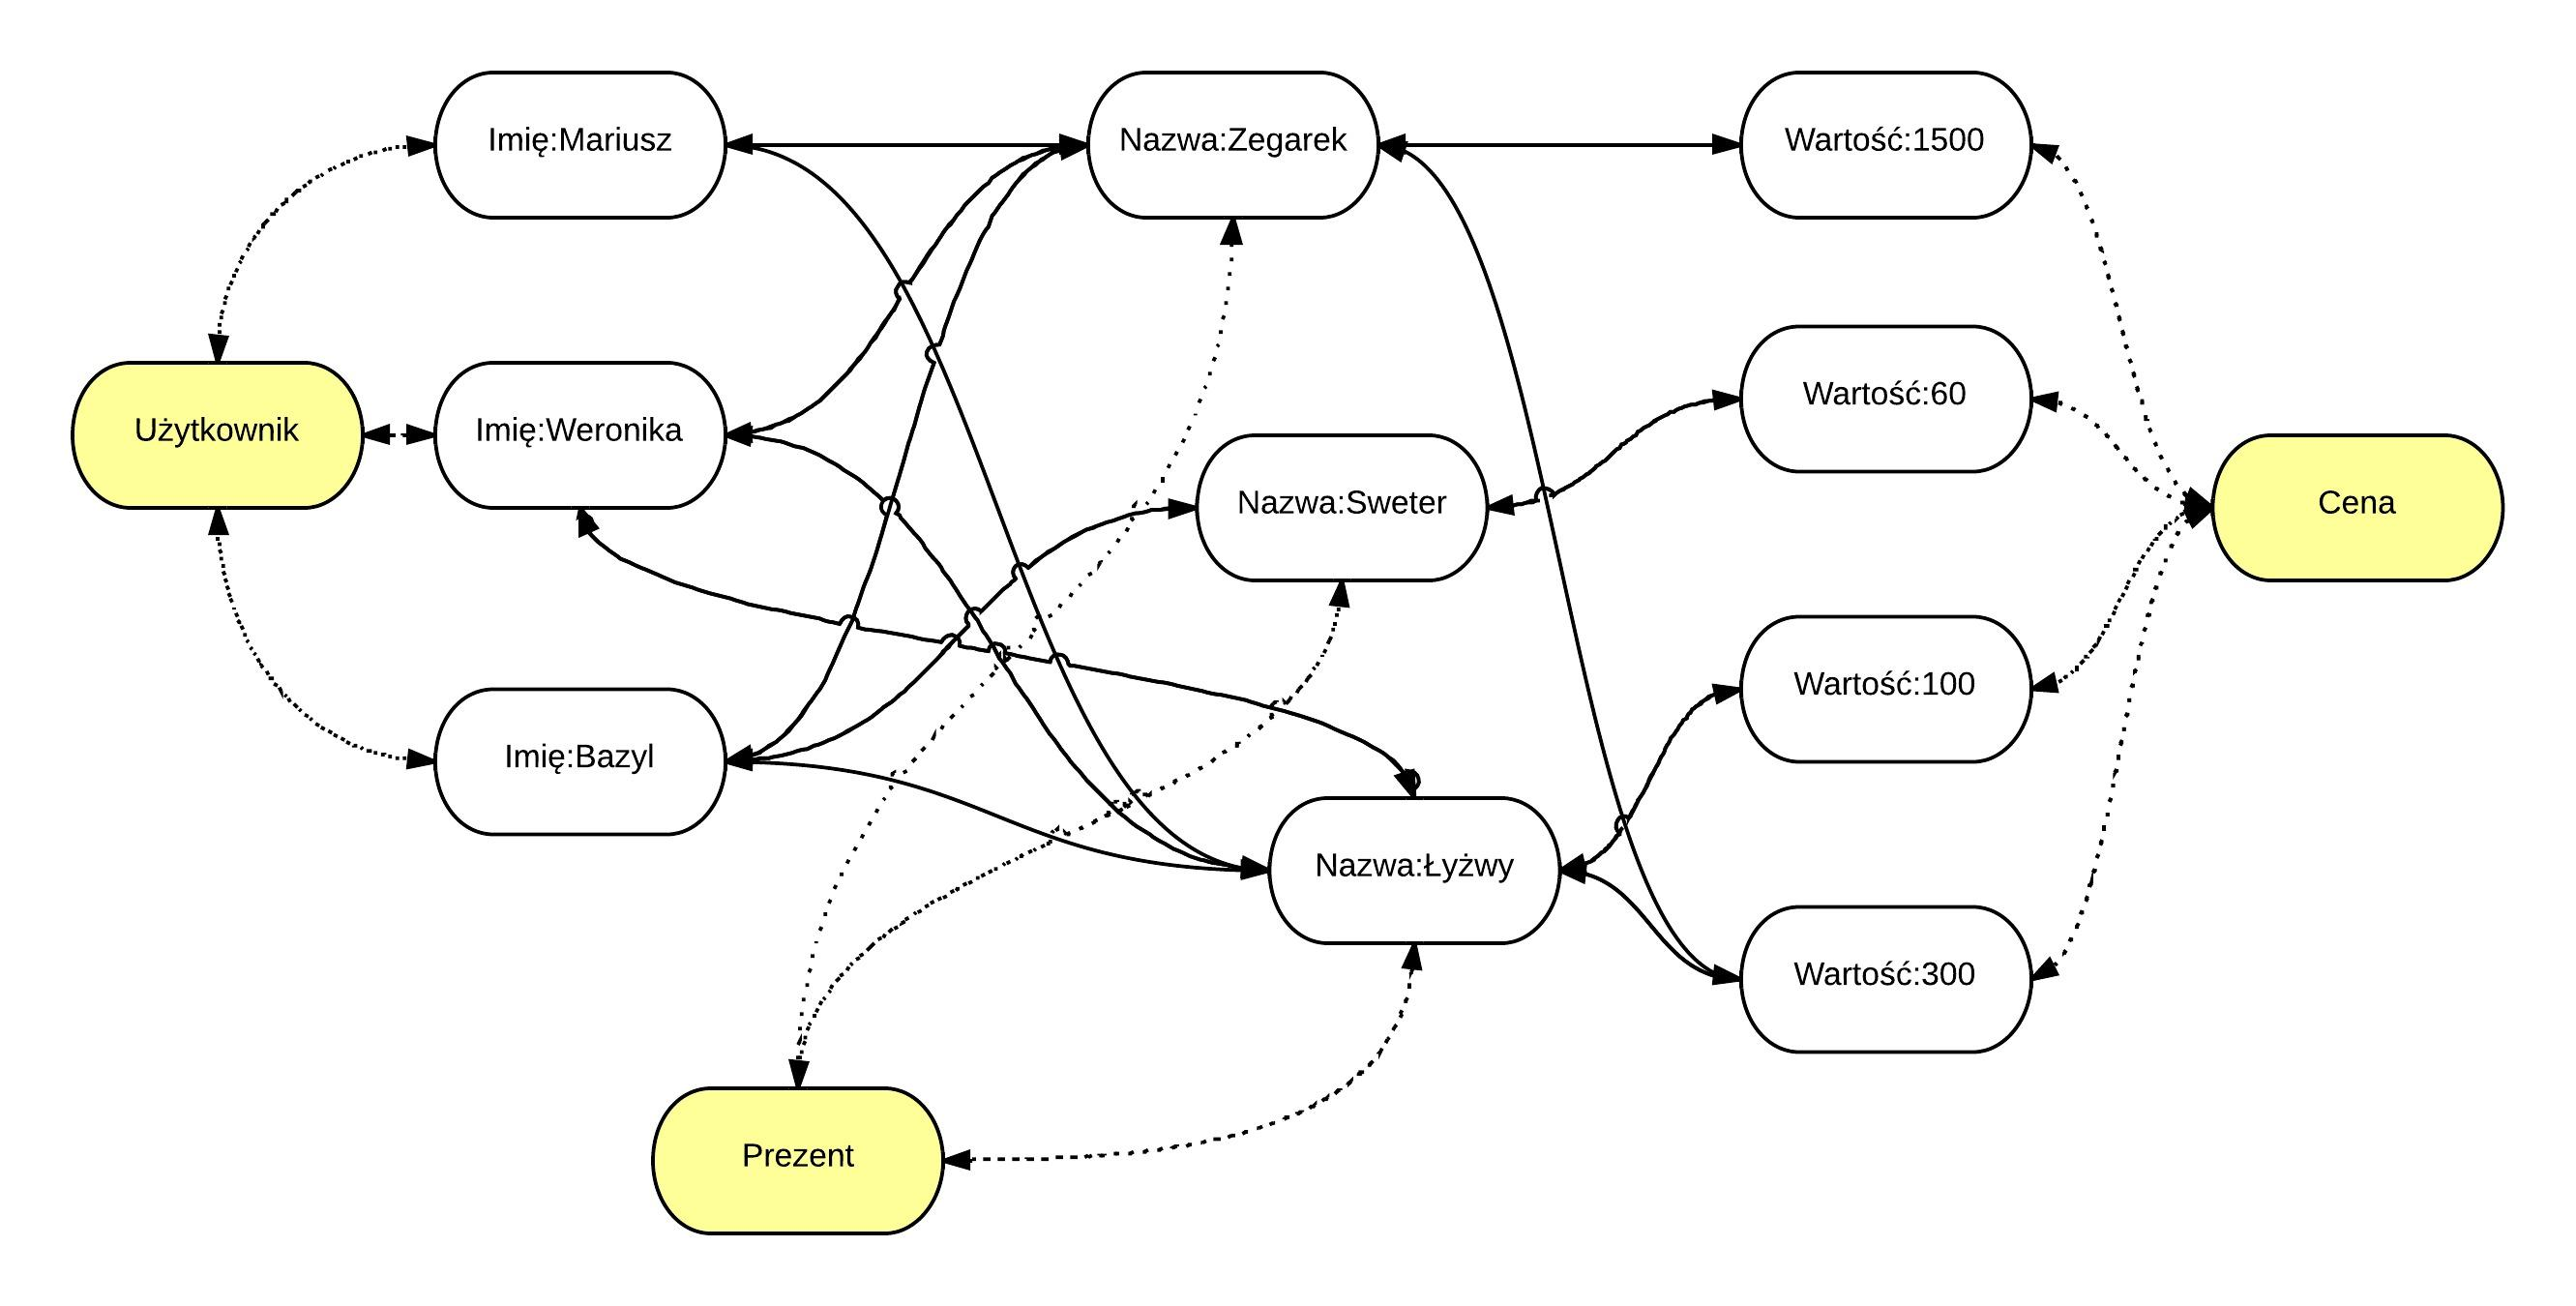
\includegraphics[width=\textwidth]{agds}
    \caption{Graf reprezentujący dane o użytkownikach i prezentach.}
\end{figure}

Zgodnie z \cite[s. 110]{Horzyk} można zauważyć, iż dostęp do każdego obiektu i jego relacji może być zrealizowany w czasie stałym \(O(1)\). W przypadku używania relacyjnych baz danych
z indeksacją za pomocą \emph{B - drzewa} - dostępną w MySQLu, czy PostreSQLu, koszt wyszukiwania wynosi \(O(log n)\). Wprawdzie można stosować index w postaci tablicy z haszowaniem, 
której średni czas dostepu wynosi \(O(1)\), jednak znacznie ogranicza to możliwości operacji na danych posiadających taki klucz.

Rysunek \ref{graph:agds}, dla przejrzystości nie uwzględnia etykietowania krawędzi grafu, ani nie przypisuje im żadnych wartości. Jednak zgodnie z definicją \ref{def:agds} nic nie stoi
na przeszkodzie, aby wprowadzic różne nazwane relacje, posiadające przypisaną im wartość, lub zbiór wartości. Dzięki temu struktury AGDS mogą być używane do przechowywania skomplikowanych,
wielopoziomowych struktur danych. Warto zwrócić uwagę również na łatwość rozszerzania istniejącej struktury o nowe typy węzłów, węzły i łączące je relacje. 

Podsumowując, struktury AGDS mogą być użyte wszędzie tam, gdzie tradycyjne struktury grafowe, dając przy tym nowe możliwości związane z modelowaniem relacji asocjacyjnych.
Szczególnie można wyróżnić następujące zastosowania \cite{Horzyk}:
\begin{itemize}
\item jako alternatywna, asocjacyjna forma reprezentacji i przechowywania danych,
\item do modelowania podstawowych asocjacyjnych relacji pomiędzy danymi,
\item do szybkiego wyszukiwannia powiązanych danych i ich kombinacji,
\item do szybkiego odnajdywania podobieństw, różnic i korelacji,
\item jako pewna forma kompresji danych i ich kombinacji,
\item jako pośrednia forma reprezentacji danych między pasywnym klasycznym oraz alternatywnym asocjacyjnym modelem przetwarzania danych.
\end{itemize}

\section{Aktywne asocjacyjne grafy neuronowe}
\label{sec:AANG}

Jedną z możliwości wykorzystania struktur AGDS jest przekształcenie ich w asocjacyjne grafy neuronowe - \textbf{AANG}. Zazwczyaj AANG nie jest używane \emph{per se}, ale dostoswywane do konkretnych aplikacji, determinując również sposób budowy grafów AGDS.

Założeniem stojącym za grafami AANG jest chęć modelowania biologicznej tkanki mózgowej. Podobnie, jak w przypadku innych sztucznych sieci neuronowych,
konieczne jest stosowanie pewnych uproszczeń, umożliwiających sprawne budowanie, uczenie i ewaluację takch struktur. W tym przypadku nacisk położony
został głównie na modelowanie odpowiedzi neuronu w czasie. Dlatego obliczanie propagacji sybału przez graf AANG polega na symulowaniu, w czasie ciągłym
lub dyskretnym, interakcji neuronów wchodzących w jej skład.

Jako, iż niniejsza praca nie skupia się w znacznym stopniu na symulacji odpowiedzi grafów AANG, wyszczególnione zostaną jedynie najważniejsze cechy neuronów asocjacyjnych.
Pełną definicję można znaleźć w \cite{Horzyk}.

\begin{definicja}
    \textbf{Asocjacyjny model neuronu - ASN} (ang. \emph{associative neuron}) jest modelem funkcjonalnym biologicznego neuronu odwzorowującym jego plastyczne zmiany w czasie oraz
    reaktywne dynamiczne sumowanie ważonych bodźców wejściowych w czasie z uwzględnieniem funkcji relaksacji i refrakcyjności. 
\end{definicja}

W dalszej częsci pracy pojęcia \emph{neuron} i \emph{neuron asocjacyjny} są stosowane zamiennie.

\begin{definicja}
    \textbf{Aktywne asocjacyjne grafy neuronowe} - \textbf{AANG}(ang. \emph{active associative neural graphs}) to pewien rodzaj sieci neuronowych
    opartych na strukturach AGDS zdolnych do aktywnego, asocjacyjnego wiązania danych, ich kombinacji i układów oraz wykonywania na nich neuroobliczeń 
    grafowych. 
\end{definicja}

Grafy AANG posiadają wszystkie zalety i cechy struktur AGDS, przy czym węzły tego grafu zamieniane są w aktywne i warunkowo reaktywe neurony, zaś krawędzie w
 asocjacyjne połączenia pomiędzy nimi. 
 
\section{Neuroasocjacyjne grafy wiedzy ANAKG}
\label{sec:anakg}

Jednym z zastosowań grafów AANG opisanych w sekcji \ref{sec:AANG} jest asocjacyjne modelowanie wiedzy. Sprowadza się ono do przetwarzania pewnego zdefiniowanego typu informacji i 
zapisywania go w postaci grafów AGDS, z możliwością przekształcenia do struktur AANG. Jest to zagadnienie szerokie i nie zostanie dogłębnie zanalizowane. Przytoczona zostanie jedynie
 część pojęć i algorytmów algorytmów, szczególnie związanych z budowaniem struktury AGDS, potrzebna do zrozumienia działania opisywanego projektu.
 
\begin{definicja}
    \label{def:wiedzaSkoj}
    \textbf{Wiedza skojarzeniowa} jest to wiedza fomułowana pod wpływem kombinacji i układów danych oraz ich sekwencji, które można zapisać w postaci \textbf{zbioru sekwencji uczących}
    $\mathbb{S}$.
\end{definicja}

Zbiór sekwencji uczących jest podstawowym nośnikiem wiedzy skojarzeniowej i może być wykorzystany do uczenia specjalnie do tego przygotowanych grafów AANG.

\begin{definicja}
    \label{def:anakg}
    \textbf{Aktywne asocjacyjne grafy wiedzy} - \textbf{ANAKG} (ang. \emph{active neuroassociative knowledge graph}) są pewnym rodzajem grafów AANG o specyficzej postaci dyskretnej
     symulacji czasu aktualizowanego w synchronicznie równoległych krokach dla wszystkich jego elementów \cite[s. 234]{Horzyk}.
\end{definicja}

Budowa grafu ANAKG zaczyna się od zdefiniowania sekwencji uczącej $S \in \mathbb{S}$ i pustego grafu ANAKG. Następnie rozpoczynana jest symulacja dyskretna z krokiem $\Delta t$, 
\begin{equation}
\label{eq:anakg}
\begin{cases}
    t_0 = 0 \\
    t_i = t_0 + \Delta t * i \\
    t_{max} = t_0 + \Delta t * card(S)
\end{cases}
\end{equation}

W chwili $t_i$ podawany jest na wejście ANAKG $i$-ty element sekwencji uczącej, powodując utworzenie lub aktywację odpowiadającego mu neuronu.
Taka aktywacja nazywana jest \textbf{aktywacją zewnętrzną}, w przeciwieństwie do \textbf{aktywacji wewnętrznej} spowodowanej sygnałami płynącymmi od
sąsiadujących neuronów. Na podstawie czasu, który upłynął między aktywacjami poszczególnych neuronów można określić tzw. \textbf{współczynnik~aktywności}W
połączenia.

\begin{definicja}
    \label{def:wspAkt}
    \textbf{Współczynnik aktywności} połączenia między neuronem presynaptycznym $SN$ akytwowanym w chwili $t_{presyn}$, a neuronem postsynaptycznym 
    $\widehat{SN}$ aktywowanym w chwili $t_{postsyn}$ definiujemy jako \cite[s. 224]{Horzyk}:
    \begin{equation}
        \begin{cases}
            \delta_{SN, \widehat{SN}}^{act} = \delta_{SN, \widehat{SN}}^{act} + \frac {1}{\tau}\\
            \tau = t_{postsyn} - t_{presyn}
        \end{cases}
    \end{equation}
\end{definicja}

Ze względu na sepcyfikę symulacji \ref{eq:anakg} stopień asocjacji ACON jest równy $\tau$. Mimo iż teoretycznie można tworzyć połączenia o dowolnym stopniu asocjacji, tj.~traktować
całą sekwencję uczącą jako jeden kontekst, proponuje się jego ograniczenie \cite{Horzyk}. Pozwala to na modelowania uogólniania i skończonej pojemności pamięci występującej
u organizmów żywych. Dzięki ograniczonemu kontekstowi zmniejsza się również komplikacja grafu i nie tworzone są powiązania pomiędzy niezwiązanymi ze sobą neuronami.

W ramach kontekstu definiowane są połączenie między następującymi po sobie neruonami. Ich wagi mogą być obliczone na podstawie zależności \cite[s. 226]{Horzyk}:

\begin{equation}
\begin{cases}
w_{SN, \widehat{SN}}^{ACON} = \frac{2 \delta_{SN, \widehat{SN}}^{act}}{\eta_{SN}^{act} + \delta_{SN, \widehat{SN}}^{act}}\\
\delta_{SN, \widehat{SN}}^{act} = \sum\limits_{(\leadsto ACON_{\tau}:SN \leadsto \dots \leadsto \widehat{SN} \in AAT)} \frac{1}{\tau}
\end{cases}
\end{equation}
gdzie 
\begin{description}
    \item $\eta_{SN}^{act}$ - ilość aktywacji neuronu $SN$ dla określonego zbioru sekwencji uczących $\mathbb{S}$.
    \item $\delta_{SN, \widehat{SN}}^{act}$ - współczynnik skuteczności połączenia synaptycznego $SN \leadsto \widehat{SN}$ (Definicja \ref{def:wspAkt}).
\end{description}

Dla zachowania integralności opisu przytoczony zostanie jeszcze wzór pozwalazjący obliczyć pobudzenie pojedynczego neuronu w chwili $t$ \cite[s. 227]{Horzyk}:

\begin{equation}
\begin{split}
\label{eq:exc}
exc_t^{SN} = NRF_{\alpha, \beta}^{SQR}(exc_{t-1}^{SN},\theta^{SN},x_1^t, \dots, x_k^t) =  \sum\limits_{k=1}^K w_k x_k^t +\\
    + \begin{cases}
    \alpha \cdot exc_{t-1}^{SN} + \frac{(\alpha - 1) \cdot \beta \cdot (exc_{t-1}^{SN})^2}{\theta^{SN}} & exc_{t-1}^{SN} < 0 \\
    \alpha \cdot exc_{t-1}^{SN} + \frac{(1 - \alpha) \cdot \beta \cdot (exc_{t-1}^{SN})^2}{\theta^{SN}} & 0 \leq exc_{t-1}^{SN} < \theta^{SN} \\
    - \beta \cdot \theta^{SN} & exc_{t-1}^{SN} \geq \theta^{SN}
    \end{cases}
\end{split}
\end{equation}
,gdzie
\begin{description}
    \item $\alpha$ reluguje szybkość relaksacji neuronu, czyli jego powracanie do stanu spoczynku. Przyjmuje się $0 \leq \alpha < 1$. Wzrost
    wartości tego współczynnika wpływa na wydłużenie okresu relaksacji.
    \item $\beta$ odpowiada za czas relaksacji neuronu w stanach podprogowych i poaktywacyjnych. Przyjmuje się $0.5 \leq \beta < 1$.
    \item $\theta^{SN}$ to próg aktywacji neuronu. Przyjmuje się $\theta = 1$.
\end{description}





 


